\documentclass{beamercours}
\title{Cours TalENS 2023-2024}
\subtitle{Inazuma Eleven, Puzzles, Angles Droits, Glissières}
\date{27 Janvier 2024}

\begin{document}
\maketitle

\section*{Introduction}
\begin{frame}
    \frametitle{Introduction Historique}
    \only<1>{\begin{figure}
        \centering
        \resizebox{8cm}{!}{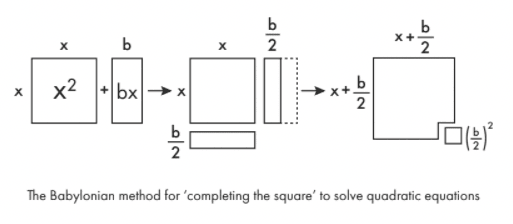
\includegraphics{Fichiers/babylonian-quadratic.png}}
        \caption{Source : \href{https://bigthink.com/hard-science/quadratic-formula-history/}{https://bigthink.com/hard-science/quadratic-formula-history/}}
    \end{figure}}

    \only<2>{\begin{figure}
        \centering
        \resizebox{8cm}{5cm}{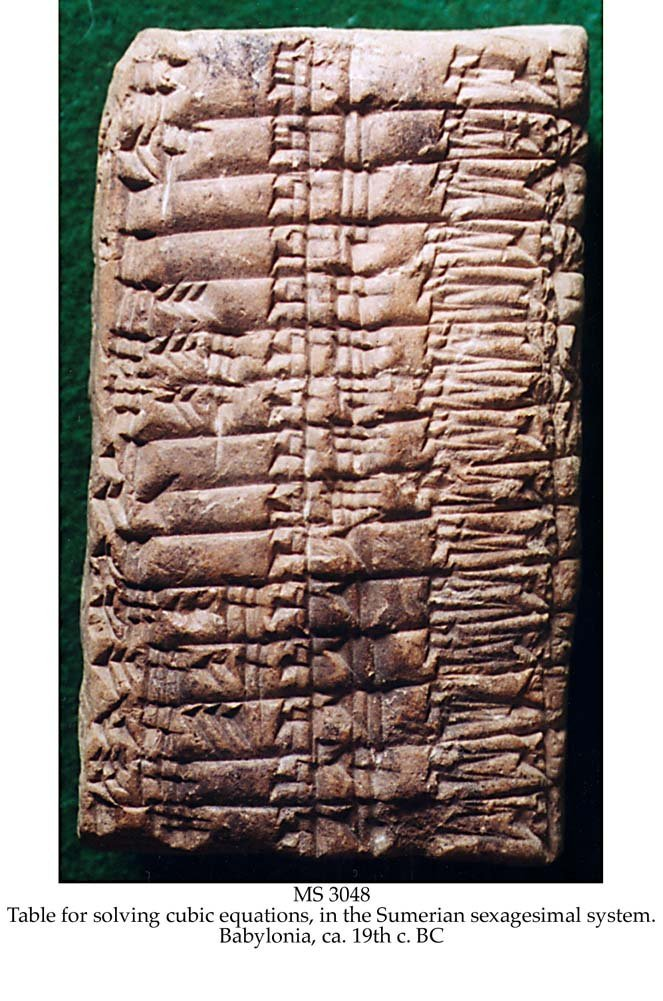
\includegraphics{Fichiers/cubic-equations-table-ms-3048_f.png}}
        \caption{Source : \href{https://www.schoyencollection.com/mathematics-collection/9-3-algebra/cubic-equations-table-ms-3048}{https://www.schoyencollection.com/mathematics-collection/9-3-algebra/cubic-equations-table-ms-3048}}
    \end{figure}}

    \only<3>{\begin{figure}
        \centering
        \resizebox{8cm}{!}{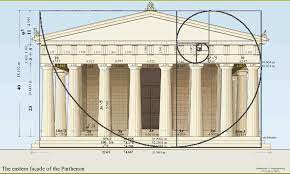
\includegraphics{Fichiers/parthenon-golden-ratio.png}}
        \caption{Source : \href{https://qph.cf2.quoracdn.net/main-qimg-a210b13c4f479bb2d8a5e4d0f1757688-lq}{https://qph.cf2.quoracdn.net/main-qimg-a210b13c4f479bb2d8a5e4d0f1757688-lq}}
    \end{figure}}
\end{frame}

\section{Formalisme !}
\subsection{Polynômes sur un Corps}
\begin{frame}
\frametitle{Le Corps}
\begin{définition}{Corps}{}
Un corps est un ensemble muni :
\begin{itemize}
    \visible<2->{\item D'une addition avec un neutre $0$ notée $+ : (x, y) \mapsto x + y$}
          \visible<3->{\item D'une multiplication avec un neutre $1$ notée $\times : (x, y) \mapsto xy$ distributive sur l'addition}
\end{itemize}
\visible<4->{Pour laquelle tout élément (sauf $0$) est inversible pour la multiplication et la loi de produit nul est vérifiée.}
\end{définition}
\visible<5>{On notera $\K$ un tel ensemble. $\R$, $\Q$, $\Z/p\Z = \mathbb{F}_{p}$ sont des corps.}
\end{frame}

\begin{frame}
\frametitle{Polynômes à une Indéterminée}
\visible<1->{\begin{définition}{Polynôme sur $\K$}{}
    Un polynôme à coefficients dans $\K$ est une suite finie d'éléments de $\K$.
    \end{définition}}
\only<2>{On les note sous la forme :
\[
    \sum_{i = 0}^{d} a_{i}X^{i}
\]}
\only<3>{On appelle le symbole $X$ l'indéterminée. Ce n'est pas un nombre. On note $\K[X]$ l'ensemble des polynômes à coefficients dans $\K$. On appelle $d$ le degré de $P$.}
\end{frame}

\begin{frame}
\frametitle{Calcul sur les Polynômes}
\only<1-3>{\begin{propositionfr}{Opérations}{}
        Si $P = \sum_{i = 0}^{d_{1}} a_{i}X^{i}$ et $Q = \sum_{j = 0}^{d_{2}} b_{j}X^{j}$ sont deux polynômes :
        \vspace{-12pt}
        \begin{itemize}[<+->]
            \item $P + Q = \sum_{i = 0}^{\max(d_{1}, d_{2})} (a_{i} + b_{i})X^{i}$ est un polynôme de degré $\leq \max(\deg P, \deg Q)$.
            \item $X^{k}P = \sum_{i = 0}^{d}a_{i}X^{i + k}$ est un polynôme.
            \item En particulier, $PQ$ est un polynôme de degré $\deg P + \deg Q$ et si $k \in \N$, $P^{k}$ est un polynôme.
        \end{itemize}
    \end{propositionfr}}
\only<4->{\begin{définition}{Composition}{}
Pour $\alpha \in \K$, on note $P(\alpha) \in \K$ le nombre : $\sum_{i = 0}^{d_{1}}a_{i}\alpha^{i}$. On note de plus $P \circ Q$ le polynôme
\[
    P \circ Q = \sum_{i = 0}^{d_{1}} a_{i}Q(X)^{i}
\]
On a $\deg P\circ Q = \deg P \times \deg Q$.
\end{définition}
La fonction $\tilde{P} : \alpha \mapsto P(\alpha)$ est continue.}
\end{frame}

\begin{frame}
\frametitle{Polynômes à Plusieurs Indéterminées}
\begin{définition}{Polynômes à Plusieurs Indéterminées}{}
Un polynôme à $k + 1$ indéterminées est un polynôme à coefficients dans $\K[X_{1}, \ldots, X_{k}]$
\end{définition}
\only<2>{\begin{remarque}{Intégrité}{}En réalité, $\K[X]$ n'est pas un corps, mais seulement un anneau intègre.\end{remarque}}
\only<3>{$P$ se met sous la forme
\[
    P(X) = \sum_{i_{1} = 0}^{d_{1}}\sum_{i_{2}=0}^{d_{2}}\ldots\sum_{i_{k} = 0} \alpha_{i_{1}, \ldots, i_{k}}X_{1}^{i_{1}}X_{2}^{i_{2}}\ldots X_{k}^{i_{k}}
\]}
\end{frame}

\subsection{Equations Polynômiales et Applications}
\begin{frame}
\frametitle{Equation Polynômiale}
\begin{définition}{Equation Polynômiale}{}
Une équation polynômiale est une équation de la forme
\[
    P(x) = \sum_{i = 0}^{d} a_{i}x^{i} = b
\]
\only<2-3>{\visible<2-3>{On peut se restreindre au cas $b = 0$ en enlevant $b$ à $P$.\\}
\visible<3>{On appelle \emph{racines} de l'équation les éléments de $\left\{\alpha \mid P(\alpha) = b \right\}$. On dit que $d = \deg P$ est le degré de l'équation. }}
\only<4->{Pour $k$ indéterminées, on remplace $x$ par un $k$-uplets $x_{1}, \ldots, x_{k}$}
\end{définition}
\end{frame}

\begin{frame}
\frametitle{Solutions à une Équation Polynômiale}
\begin{propositionfr}{Nombres de Solution}{}
    Une équation définie par $P$ a au plus $\deg P$ solutions
\end{propositionfr}
\visible<2->{\begin{théorème}{D'Alembert Gauss}{}
    Une équation polynômiale définie par $P$ a toujours exactement $\deg P$ solutions sur un corps algébriquement clos. $\C$ est algébriquement clos.
    \end{théorème}}
\end{frame}

\begin{frame}
\frametitle{Applications I}
\begin{définition}{Droite}{}
Une droite est un ensemble de la forme $D(a, b) = \{ax + b \mid x \in \R\}$
\end{définition}

\visible<2->{En particulier, si on a deux droites $D(a, b), D(a', b')$, leur intersection est définie par l'ensemble
    \[
        \left\{ax + b = a'x + b'\right\} = \left\{(a - a')x + (b - b') = 0\right\}
    \]}
\end{frame}

\begin{frame}
\frametitle{Applications II}
\begin{définition}{Cercle}{}
Un cercle est un ensemble de la forme $C((x_{0}, y_{0}), r) = \left\{(x - x_{0})^{2} + (y - y_{0})^{2} = r^{2}\right\}$
\end{définition}
De la même manière que pour les droites, on peut vérifier que les points à l'intersection de deux cercles sont solutions d'une équation polynomiale.
\end{frame}

\section{Algorithmes}
\subsection{Analyse des Algorithmes}
\begin{frame}
\frametitle{Notion de Complexité}
\visible<1->{
    \begin{définition}{Complexité}{}
    On appelle complexité en temps d'un algorithme le nombre d'opérations nécessaires à l'effectuer.
    \end{définition}
    La complexité est une notion de vitesse d'un algorithme.}
\visible<2->{
    \begin{définition}{Notation de Landau}{}
    On dit que $u_{n} = \O(v_{n})$ si il existe $c$ tel que $\frac{u_{n}}{v_{n}} \leq c$ pour tout $n$.
    \end{définition}
    \vspace{-5pt}
    La notation \texttt{grand O} est une notion de vitesse de croissance.}
\end{frame}
\begin{frame}
    \frametitle{Quelques Exemples}
    \begin{propositionfr}{Croissances Comparées}{}
        \begin{itemize}[<+->]
            \item On a $\alpha^{n} = \O\left(\beta^{n}\right)$ si $0 \leq \alpha \leq \beta$
            \item On a $n^{\alpha} = \O\left(n^{\beta}\right)$ si $0 \leq \alpha \leq \beta$
            \item A l'inverse $n^{\alpha} = \O\left(n^{\beta}\right)$ avec $\alpha \leq \beta\leq 0$
            \item On a $\log n \leq n^{\alpha}$ si $\alpha > 0$.
        \end{itemize}
    \end{propositionfr}
\end{frame}

\begin{frame}
    \frametitle{Propriétés}
    \begin{propositionfr}{Opérations}{}
        Si $u_{n} = \O(v_{n})$
        \begin{itemize}
            \item<2-> Si $v_{n} = \O\left(w_{n}\right)$ on a $u_{n} = \O(w_{n})$
            \item<3-> $\lambda u_{n} = \O(v_{n}) = \O(\lambda v_{n})$
            \item<4-> Si $w_{n} = \O(z_{n})$ on a : $u_{n} + w_{n} = \O(v_{n} + z_{n})$.
            \item<5-> $u_{n} = \O(u_{n})$.
        \end{itemize}
    \end{propositionfr}
\end{frame}

\subsection{Algorithmes sur les Polynômes}
\begin{frame}
    \frametitle{Algorithmes Simples}
    \only<1>{\begin{tabular}{m{.5\linewidth}m{.45\linewidth}}
            Algorithme                                                                   & Analyse \\
            \midrule{
            \begin{algorithmic}
                    \Input\  $P = \left(a_{0}, \ldots, a_{n}\right)$, \newline $Q = \left(b_{i}, \ldots, b_{n}\right)$
                    \EndInput
                    \State Calculer les puissances de $x$ jusqu'à $n$
                    \State Calculer $a_{i}x^{i}$
                    \State \Return Somme des résultats
                \end{algorithmic}} &
            On effectue $n$ additions, on a une complexité en $\O(n)$.                             \\
        \end{tabular}}
    \only<2->{\begin{tabular}{m{.5\linewidth}m{.45\linewidth}}
            Algorithme                                                                 & Analyse                        \\
            \midrule
            \begin{algorithmic}
                \Input\  $P = \left(a_{0}, \ldots, a_{n}\right)$\newline $Q = \left(b_{i}, \ldots, b_{n}\right)$
                \EndInput
                \State Calculer les puissances de $x$ jusqu'à $n$
                \State Calculer $a_{i}x^{i}$
                \State \Return Somme des résultats
            \end{algorithmic} & On effectue $n$ produits par puissance, donc a une complexité en $\O\left(n^{2}\right)$
        \end{tabular}
        \visible<3->{En réalité, il existe un algorithme plus efficace pour calculer un produit de polynômes, appelé \textsc{Fast Fourier Transform}, et celui-ci fonctionne en $\O(n\log{n})$.}
    }
\end{frame}

\begin{frame}
    \frametitle{Evaluation Naïve}
    \begin{tabular}{m{.5\linewidth}m{.45\linewidth}}
        Algorithme                                            & Analyse \\
        \midrule{
        \begin{algorithmic}
                \Input\  $P = \left(a_{0}, \ldots, a_{n}\right)$, $x$
                \EndInput
                \State Calculer les puissances de $x$ jusqu'à $n$
                \State Calculer $a_{i}x^{i}$
                \State \Return Somme des résultats
            \end{algorithmic}} &
        \only<1>{De manière naïve, on calcule $x^{i}$ en temps $\O(i)$. On a alors une complexité en $\O(n^{2})$.\newline}
        \only<2->{Sans rentrer dans les détails, on peut calculer $x^{i}$ en temps $\log(i)$. On fait donc un nombe d'opérations en $\O(n\log n)$.}
    \end{tabular}
\end{frame}

\begin{frame}
    \frametitle{Algorithme de Horner}
    \begin{propositionfr}{Evaluation Rapide de Horner}{}
        \vspace{-18pt}
        \[\begin{split}
                P(X) = \sum_{k = 0}^{n}a_{k}X^{k} &= (\left(\left(a_{n} \times X + a_{n - 1}\right)\right.\\
                &\left.\hspace{2cm} \times X + a_{n - 2}\right)\\
                & \hspace{3cm} \ldots + a_{1})\times X + a_{0}
            \end{split}\]
    \end{propositionfr}
    \visible<2>{De ceci, on déduit un algorithme d'évaluation des polynômes en $n$ multiplications et $n$ additions!}
\end{frame}

\section{Résolution des Equations}
\subsection{Formellement}
\begin{frame}
\frametitle{Degrés $1$ et $2$}
\vspace{-5pt}
\begin{théorème}{Solution des Equations Affines}{}
L'unique solution de $ax + b = c$ avec $a \neq 0$ est $x = \frac{c - b}{a}$
\end{théorème}
\vspace{-8pt}
\visible<2->{\begin{théorème}{Solution des Equations Quadratiques}{}
    Les deux solutions de $ax^{2} + bx + c = d$ avec $a \neq 0$ sont :
    \vspace{-6pt}
    \[
        x_{+} = \frac{- b + \sqrt{b^{2} - 4a(c - d)}}{2a} \text{ et } x_{-} = \frac{- b - \sqrt{b^{2} - 4a(c - d)}}{2a}
    \]
    Celles-ci ne sont réelles que si $\sqrt{b^{2} - 4a(c - d)} \geq 0$ et sont égales s'il y a égalité. Sinon, elles sont complexes conjuguées.
    \end{théorème}}
\end{frame}
\begin{frame}
\frametitle{Degrés $3$, $4$ et plus}
\begin{théorème}{Solutions des Cubiques et Quartiques}{}
Il existe des formules pour les solutions des équations de la forme $ax^{3} + bx^{2} + cx + d = e$ et $ax^{4} + bx^{3} + cx^{2} + dx + e = f$ où $a \neq 0$. Ces racines ne sont pas toujours réelles, mais une équation de degré trois a toujours une racine réelle.
\end{théorème}
\visible<2->{\begin{théorème}{Klein Vierergruppe}{}
    Il ne peut pas exister de formule pour les solutions des équations polynômiales de degré $\geq 5$.
    \end{théorème}}
\end{frame}

\subsection{Méthodes de Résolution Graphique}
\begin{frame}
\frametitle{Théorème des Valeurs Intermédiaires}
\begin{théorème}{des Valeurs Intermédiaires}{}
\begin{itemize}[<+->]
    \item Formulation Réelle : Si $f$ est continue sur un intervalle, son image est un intervalle.
    \item Formulation Générale : Si $f$ est continue sur le connexe par arcs $X$, son image est connexe par arcs.
\end{itemize}
\end{théorème}
\visible<3->{En pratique cela signifie que si:
    \[
        f(a) = c, f(b) = d \text{ alors } \forall y \in \left[c, d\right], \exists x, f(x) = y
    \]}
\end{frame}

\begin{frame}
\frametitle{Méthode de Newton-Raphson}
\begin{théorème}{Caractérisation de Carathéodory}{}
Une fonction est dérivable en $x_{0}$ si et seulement si il existe un nombre noté $f'(x_{0})$ tel que, au voisinage de $x_{0}$ :
\[
    f(x) = f(x_{0}) + f'(x)(x- x_{0})
\]
\end{théorème}
\visible<2->{En particulier, les polynômes sont dérivables, donc si on cherche une racine $x_{0}$, on peut, en suivant la pente, trouver une racine.\\}
\visible<3->{Si $f(x) > 0$ et on va selon $x$ croissant si $f(x) < 0$ sinon $x$ décroissant et à l'inverse sinon.}
\end{frame}
\begin{frame}
    \frametitle{Méthode de Newton-Raphson Graphique}
    \begin{tabular}{m{.55\linewidth}m{.4\linewidth}}

        \begin{tikzpicture}
            \draw[very thin, color = vulm] (-1.1, -1.1) grid (2.9, 2.9);
            \draw[->, vulm] (-1.2,0) -- (3.2,0) node[right] {$x$};
            \draw[->, vulm] (0,-1.2) -- (0,3.2) node[above] {$f(x)$};
            \draw[color = vulm, domain = -1:2.5] plot (\x, {\x^2 -\x - 1}) node[above] {$f(x) = x^{2} - x - 1$};
            \draw[color = black] (2.2, 1.64) node {\bf x};
            \draw[->, color = black] (2.4, 2.32) -- node[right] {$f'(x) = +3.4$} (1.8,.28) ;
        \end{tikzpicture} &
        \visible<2->{On vérifie bien qu'on va trouver une racine en \[\phi = \frac{1 + \sqrt{5}}{2}\]}
        \visible<3->{Il y en a une autre en \[ \overline{\phi} = \frac{1 - \sqrt{5}}{2} \]}
    \end{tabular}
    \visible<3->{Toutefois, cette méthode graphique nécessite de savoir tracer une fonction polynômiale.}
\end{frame}

\end{document}
